\section{Architekturen}
\label{subsec:architekturen}
Da Blazor in zwei Varianten existiert, existieren dementsprechend auch zwei Architekturen für
dieses Framework. Bevor die zwei Architekturen jedoch im Detail erklärt werden, sollte zuerst ein
grundlegendes wissen darüber veranschaulicht werden, wie bis jetzt andere \ac{spa}, wie zum
Beispiel Angular oder React sowas gehandhabt haben. Die heutigen \ac{spa} basieren auf der
Client-Server Architektur, das bedeutet der Client stellt eine Anfrage an den Server und erhält
dann, sollte alles stimmen, die passende Antwort. Die Kommunikation der beiden Teilnehmer
geschieht dann in den meisten Fällen über eine REST Api. Heutzutage gibt es noch andere
Alternativen zu REST, wie zum Beispiel gRPC, jedoch ist bis heute der Standard für die
Kommunikation noch REST.
In dem folgenden Schaubild ist eine solche Architektur zu sehen:
\begin{figure}[h]
    \centering
    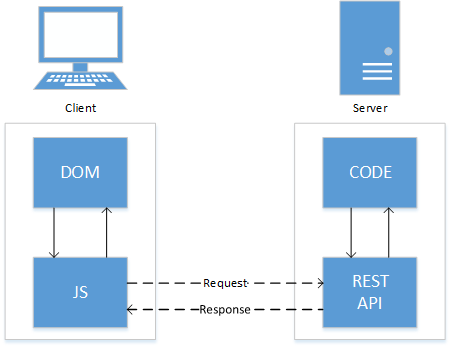
\includegraphics[width=0.7\textwidth, center]{StandDerTechnik/ClientServerJS}
    \caption[Client-Server Architektur mit Javascript]{Client-Server Architektur mit Javascript}
    \label{img:clientserverjs}
\end{figure}

Wie zu sehen ist, Kommuniziert der Client mithilfe von Javascript mit dem Server. Javascript holt
sich also die Daten, welche der Client braucht und gibt diese dem DOM zum verarbeiten weiter.

\subsection{Blazor WebAssembly}
Bei Blazor WebAssembly ist es so, dass sich die Architektur von den anderen \ac{spa} wie Angular
nicht groß verändert. Tatsächlich verändert sich hierbei nur die Programmiersprache, die auf dem
Client läuft. Es handelt sich dabei um die Programmiersprache C\#, die dann auf dem Client
ausgeführt wird, wie im folgenden zu sehen ist.
\begin{figure}[h]
    \centering
    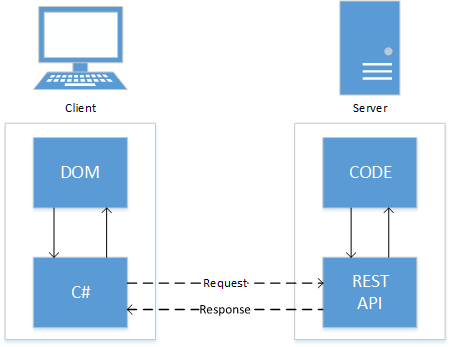
\includegraphics[width=0.7\textwidth, center]{StandDerTechnik/ClientServerCsharp}
    \caption[Blazor WebAssembly Architektur]{Blazor WebAssembly Architektur}
    \label{img:clientservercsharp}
\end{figure}
\newline
\newline
Das ganze Konzept C\# überhaupt auf dem Client laufen lassen zu können, funktioniert durch
WebAssembly. WebAssembly wandelt Programmcode in nativen Bytecode um, der dann in einer Sandbox
im Browser ausgeführt werden kann. Dabei wird von der Sandbox aus die DOM mit hilfe von
Javascript kontinuierlich manipuliert. Javascript verschwindet in dem Sinne also nicht komplett
sondern wird lediglich ergänzt.
Da für dieses Konzept als WebAssembly vonnöten ist, kann Blazor WebAssembly nicht auf Browsern
funktionieren, die WebAssembly nicht unterstützen \cite{HierKommtBlazor}[vgl.].
\newline
\newline
Im folgenden werden noch die Vor- und Nachteile von Blazor WebAssembly dargestellt:
\begin{itemize}
    \pro Sehr Skallierbar
    \pro Sehr Performant
    \pro Es kann komplett eigenständig auf dem Client laufen und ist nicht unbedingt auf dem
    Server angewiesen
    \con Große Anwendungsdatei, die komplett auf dem Client geladen werden muss
    \con Lange ladezeit beim ersten Aufruf
    \con Kompletter Code ist auf dem Client zu sehen
\end{itemize}

\subsection{Blazor Server}
Anders als es bei Blazor WebAssembly der Fall ist, wird bei Blazor Server nicht C\# in den
Browser geladen, sondern das ganze Konzept spielt sich auf dem Server ab. Deswegen wird auch die
Web-Anwendung als SPA auf dem Server gerendert. Zum Client werden nur JavaScript und Markup
gesendet und die Daten und Benutzereingaben laufend mittels SignalR zwischen Client und Server
ausgetauscht. Dementsprechend ist es auch vonnöten, dass immer zwischen dem Client und dem Server
eine offene Verbindung vorhanden ist \cite{HierKommtBlazor}[vgl.].
\newline
\newline
Dadurch das die komplette Seite auf dem Server gerendert wird, lädt die Seite auf dem Client sehr
schnell, muss nur eine kleine Javascript Datei auf den Client laden und kann auf sehr
Leistungsschwachen Clients verwendet werden. Zudem kommt auch noch, anders als bei Blazor
WebAssembly, dass sich jeder Browser verwenden lässt unabhängig davon ob dieser WebAssembly
unterstützt oder nicht.
\newline
\newline
Das ganze Konzept dieser Architektur, baut drauf auf, dass beim ersten Aufruf der Seite eine
Javascript Datei names \emph{Blazor.js} auf dem Client geladen wird. Diese Daten kommuniziert dann mit
dem DOM und baut die Verbindung zum Server auf. Sobald die Verbindung aufgebaut ist, werden
kontinuierlich Nachrichten zwischen Client und Server ausgetauscht, wie im folgenden zu sehen ist:
\begin{figure}[h]
    \centering
    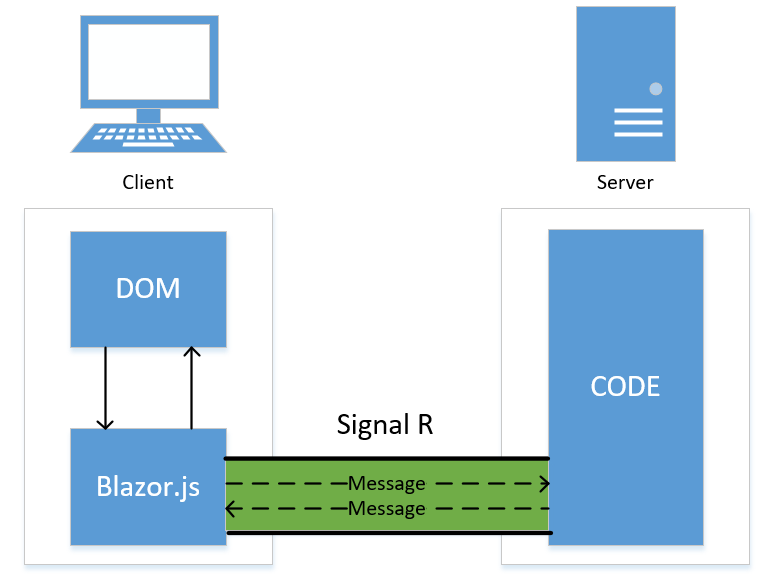
\includegraphics[width=0.7\textwidth, center]{StandDerTechnik/ClientServerSignalR}
    \caption[Blazor Server Architektur]{Blazor Server Architektur}
    \label{img:clientserversignalR}
\end{figure}

Im folgenden werden noch die Vor- und Nachteile von Blazor Server zusammengestellt:
\begin{itemize}
    \pro Kurze Ladezeiten
    \pro Es ist komplett Browserunabhängig
    \pro Client hat keinen Zugriff auf den SourceCode
    \con Nicht Skallierbar, da alle Benutzer auf einem Server zugreifen
    \con Lange Netzwerklatenz führt zu Verzögerungen in der Benutzeroberfläche
    \con Es muss immer eine Verbindung bestehen
\end{itemize}